%%%%%%%%%%%%%%%%%%%%%%%%%%%%%%%%%%%%%%%%%
% University Assignment Title Page 
% LaTeX Template
% Version 1.0 (27/12/12)
%
% This template has been downloaded from:
% http://www.LaTeXTemplates.com
%
% Original author:
% WikiBooks (http://en.wikibooks.org/wiki/LaTeX/Title_Creation)
%
% License:
% CC BY-NC-SA 3.0 (http://creativecommons.org/licenses/by-nc-sa/3.0/)
% 
% Instructions for using this template:
% This title page is capable of being compiled as is. This is not useful for 
% including it in another document. To do this, you have two options: 
%
% 1) Copy/paste everything between \begin{document} and \end{document} 
% starting at \begin{titlepage} and paste this into another LaTeX file where you 
% want your title page.
% OR
% 2) Remove everything outside the \begin{titlepage} and \end{titlepage} and 
% move this file to the same directory as the LaTeX file you wish to add it to. 
% Then add \input{./title_page_1.tex} to your LaTeX file where you want your
% title page.
%
%%%%%%%%%%%%%%%%%%%%%%%%%%%%%%%%%%%%%%%%%
%\title{Title page with logo}
%----------------------------------------------------------------------------------------
%	PACKAGES AND OTHER DOCUMENT CONFIGURATIONS
%----------------------------------------------------------------------------------------

\documentclass[12pt]{article}
\usepackage[italian]{babel}
\usepackage[utf8x]{inputenc}
\usepackage{amsmath}
\usepackage{graphicx}
\usepackage[colorinlistoftodos]{todonotes}

\begin{document}
	\begin{titlepage}
	
	\newcommand{\HRule}{\rule{\linewidth}{0.5mm}} % Defines a new command for the horizontal lines, change thickness here
	
	\center % Center everything on the page
	
	%----------------------------------------------------------------------------------------
	%	HEADING SECTIONS
	%----------------------------------------------------------------------------------------
	
	\textsc{\LARGE Università degli studi di Padova}\\[1.5cm] % Name of your university/college
	
\includegraphics[scale=0.3]{images/unipd_logo.png}\\[1cm] % Include a department/university logo - this will require the graphicx package
	\textsc{\Large Relazione progetto per il corso di tecnologie web}\\[0.5cm] % Major heading such as course name
	\textsc{\large Corso di Laurea in Informatica, A.A. 2016-2017}\\[0.5cm] % Minor heading such as course title
	%----------------------------------------------------------------------------------------
	%	TITLE SECTION
	%----------------------------------------------------------------------------------------
	
	\HRule \\[0.4cm]
	{ \huge \bfseries ASTROPORT}\\[0.4cm] % Title of your document
	\HRule \\[1.5cm]
	
	%----------------------------------------------------------------------------------------
	%	AUTHOR SECTION
	%----------------------------------------------------------------------------------------
	
	\begin{minipage}{0.4\textwidth}
	\begin{flushleft} \large
	\emph{Studenti:}\\
	Mattia Bottaro \#1097723 \\--------\\ Andrea Magnan \#1096609 \\--------\\ Riccardo Saggese \#1051333 \\--------\\ Matteo Slanzi \\ \#1100866
	\end{flushleft}
	\end{minipage}
	~
	\begin{minipage}{0.4\textwidth}
	\begin{flushright} \large
	\emph{Docente:} \\
	Ombretta Gaggi
	\end{flushright}
	\end{minipage}\\[2cm]
	
	% If you don't want a supervisor, uncomment the two lines below and remove the section above
	%\Large \emph{Author:}\\
	%John \textsc{Smith}\\[3cm] % Your name
	
	%----------------------------------------------------------------------------------------
	%	DATE SECTION
	%----------------------------------------------------------------------------------------
	
	%{\large \today}\\[2cm] % Date, change the \today to a set date if you want to be precise
	
	%----------------------------------------------------------------------------------------
	%	LOGO SECTION
	%----------------------------------------------------------------------------------------
	
	
	%----------------------------------------------------------------------------------------
	
	\vfill % Fill the rest of the page with whitespace
	
	\end{titlepage}
	\newpage
	\section{Informazioni utili}
	\textsc{\Large Link al sito\\ }link\\[0.5cm]
	\textsc{\Large Mail del referente:\\ }mattia.bottaro@studenti.unipd.it\\[0.5cm]
	\textsc{\Large Login User:}\\[0.5cm] mail: user, password: user 
	\newpage
	\tableofcontents
	\listoffigures
	\listoftables
	\newpage
	
	
	\section{Abstract}
	Il progetto sviluppato si propone di implementare un sito che ha come scopo quello di divulgare i principali eventi astronomici osservabili dalla terra.
	Il sito vuole quindi essere un riferimento per gli astrofili, i quali potranno consultare studi e foto, oltre a informarsi sugli eventi astronomici passati e futuri. \\
	Le categorie di utenti che possono utilizzare il sito sono:
	\begin{itemize}
	\item utenti non loggati;
	\item utenti loggati.
	\end{itemize}
	Il sito è stato sviluppato rispettando gli
	standard W3C, la separazione tra struttura, presentazione, comportamento
	e le regole di accessibilità richieste.
	
	\section{Materiale Consegnato}
	\section{Il sito}
	
	Il sito si propone di:
	\begin{itemize}
		\item permettere la consultazione degli studi(foto) presenti nel DB a tutti gli utenti;
		\item permettere la votazione e/o commentare gli studi(foto) presenti nel DB ai soli utenti loggati;
		\item fornire a tutti gli utenti le date dei principali eventi astronomici, passati e futuri.
	\end{itemize}
	\section{Utenti destinatari}
	Come anticipato nell'\textit{Abstract}, gli utenti destinatari del sito sono tutte quelle persone che hanno un qualche interesse per l'astronomia.
	In particolare, miriamo a:
	\begin{itemize}
		\item utenti che hanno interesse nel sapere quali eventi astronomici ci saranno(o ci sono stati), in quanto nel sito è presente una lista che soddisfa questa esigenza;
		\item utenti che vogliono imparare qualcosa dell'astronomia, in quanto il sito offre alcuni studi divulgativi su certi eventi astronomici e/o certi corpi celesti.
		\item utenti che vogliono semplicemente guardare qualche bella foto del cielo, in quanto il sito offre diverse foto alcune delle quali consultabili tramite uno slideshow nella home page.
		
	\end{itemize}
	\section{Accessibilità}
	\subsection{Separazione contenuto, struttura e presentazione}
	\subsection{Schema colori}
	Lo schema dei colori adottato mira a dare meno disagi possibili agli utenti affetti da particolari patologie agli occhi, quali deuteranopia, protanopia e tritanopia. Gli screenshot qui sotto sono una simulazione di come un utente appartenente a questa categoria vede il nostro sito.\\
	\begin{figure}
		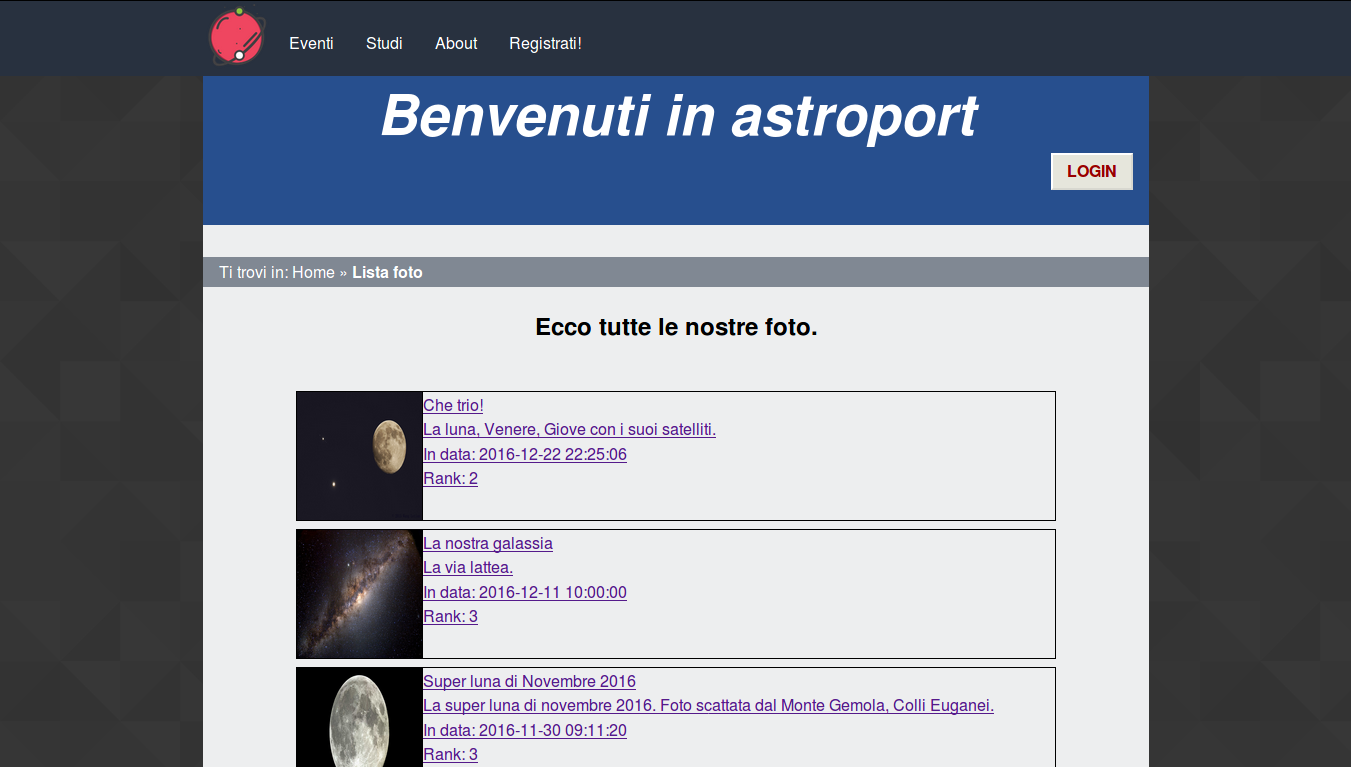
\includegraphics[scale=0.3]{images/test.png}\\[1cm] \caption{pagina lista delle foto vista da un utente normale.}
	\end{figure}
	\begin{figure}
		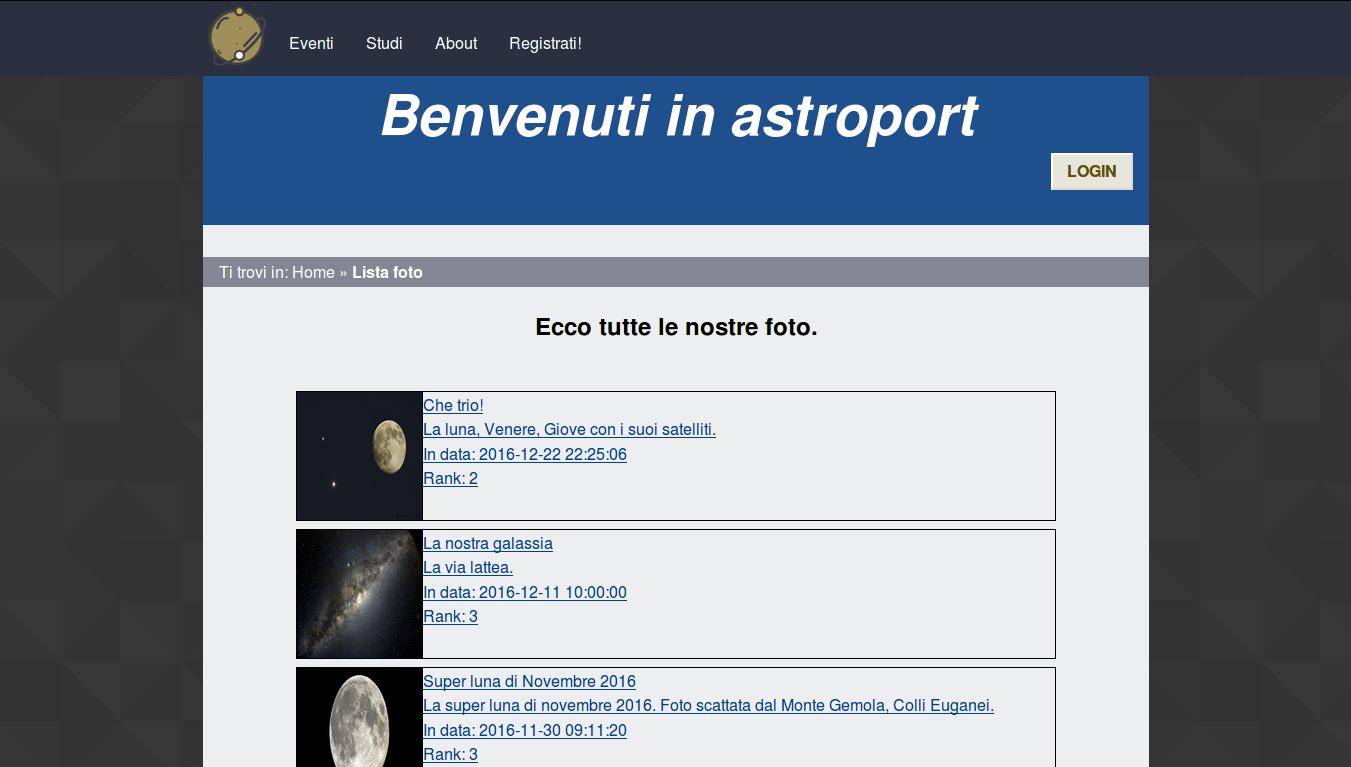
\includegraphics[scale=0.3]{images/deuteranopia.jpg}\\[1cm] \caption{Utente affetto da deuteranopia}
	\end{figure}
	\begin{figure}
		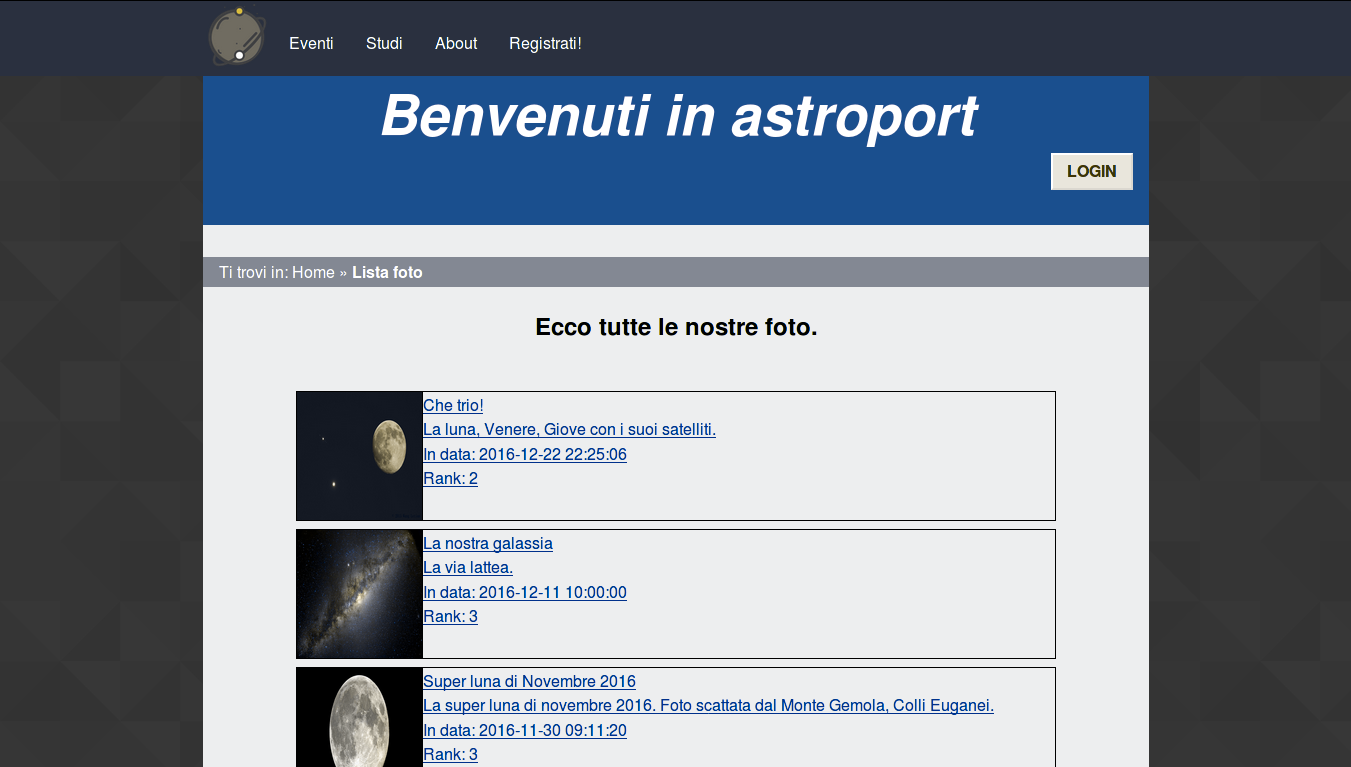
\includegraphics[scale=0.3]{images/protanopia.jpg}\\[1cm] \caption{Utente affetto da protanopia}
	\end{figure}
	\begin{figure}
		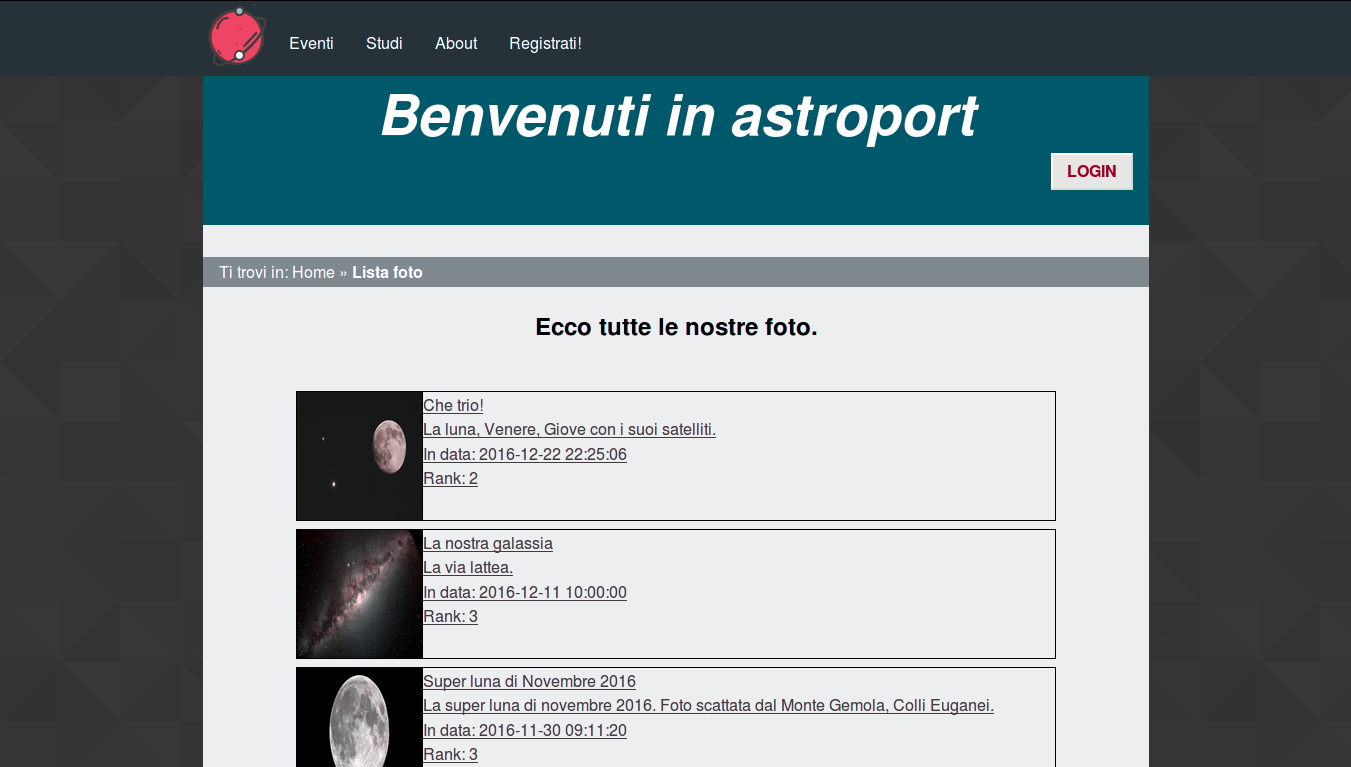
\includegraphics[scale=0.3]{images/tritanopia.jpg}\\[1cm] \caption{Utente affetto da tritanopia}
	\end{figure}
	\begin{figure}
		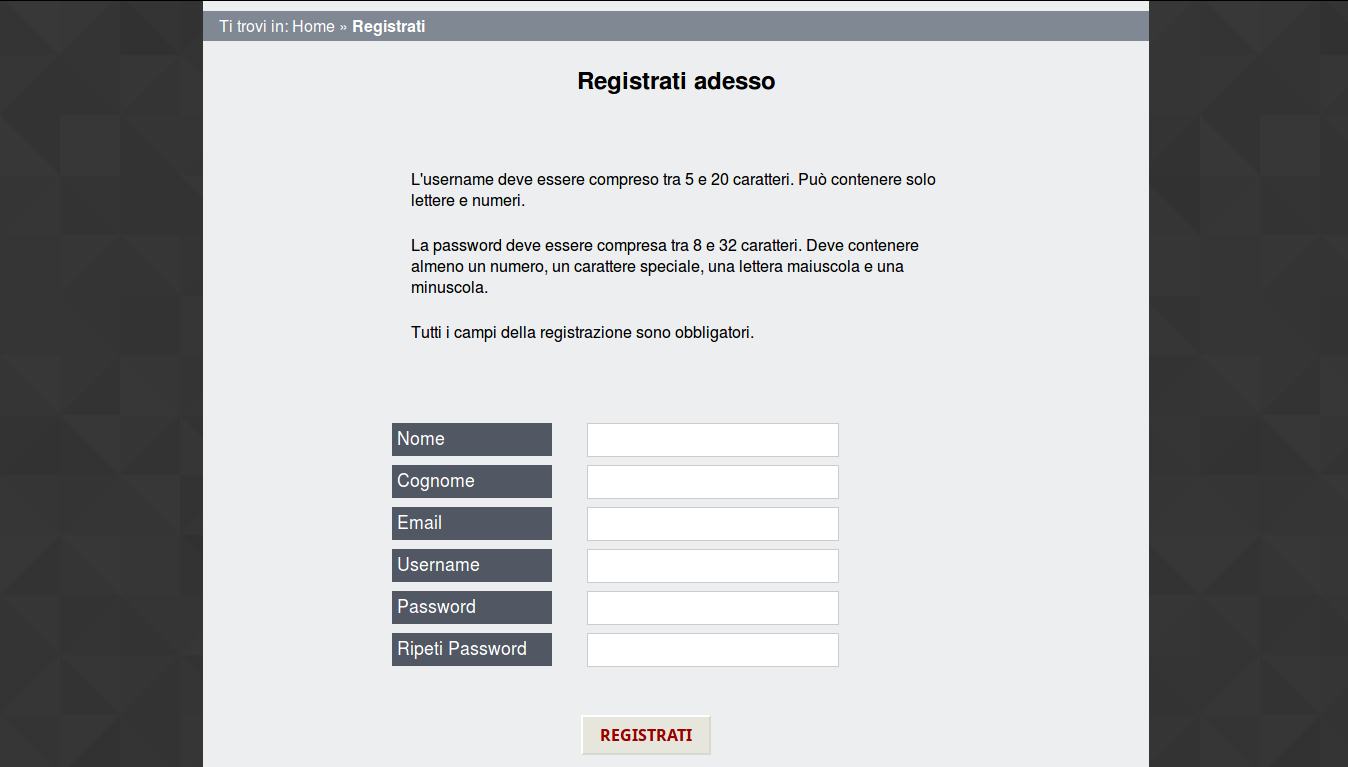
\includegraphics[scale=0.3]{images/test2.png}\\[1cm] \caption{pagine per la registrazione al sito vista da un utente normale} \end{figure}
	\begin{figure}
		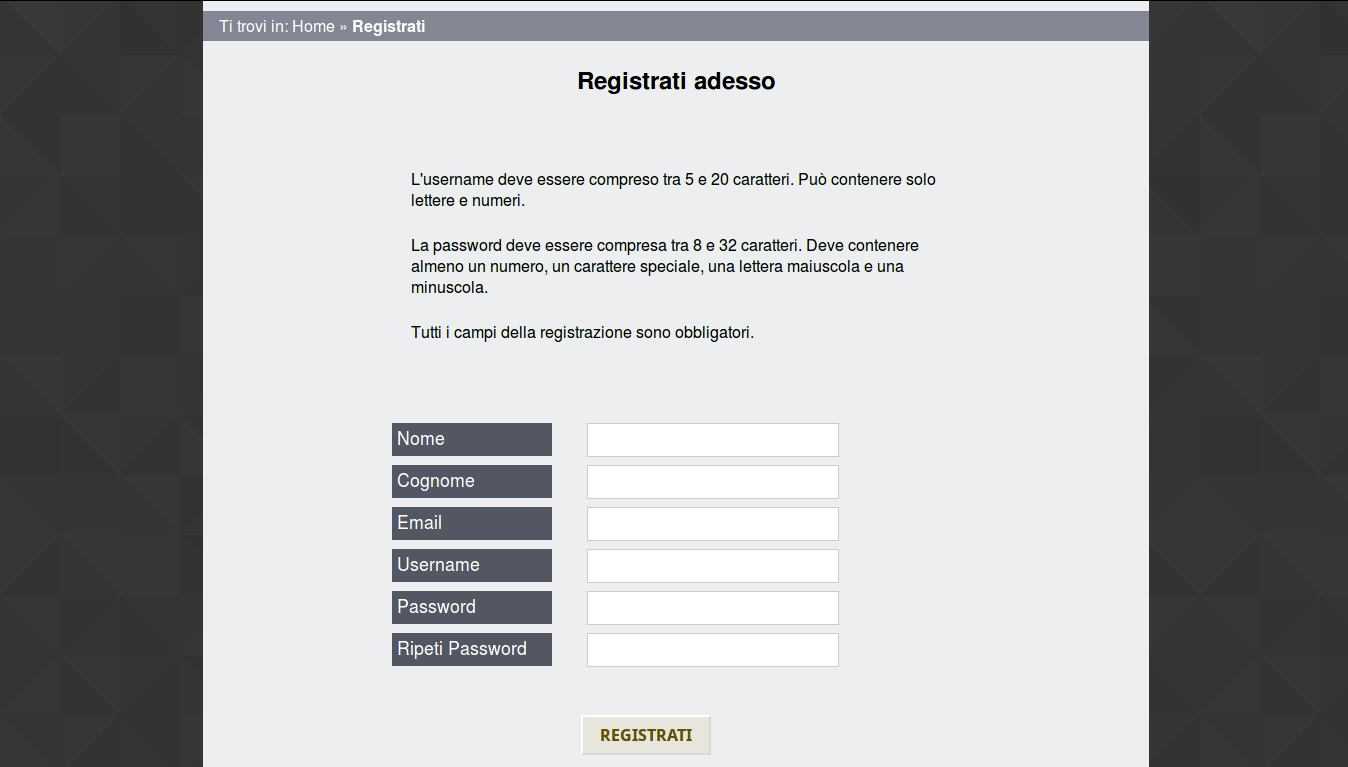
\includegraphics[scale=0.3]{images/deuteranopia2.jpg}\\[1cm] \caption{Utente affetto da deuteranopia}
	\end{figure}
	\begin{figure}
		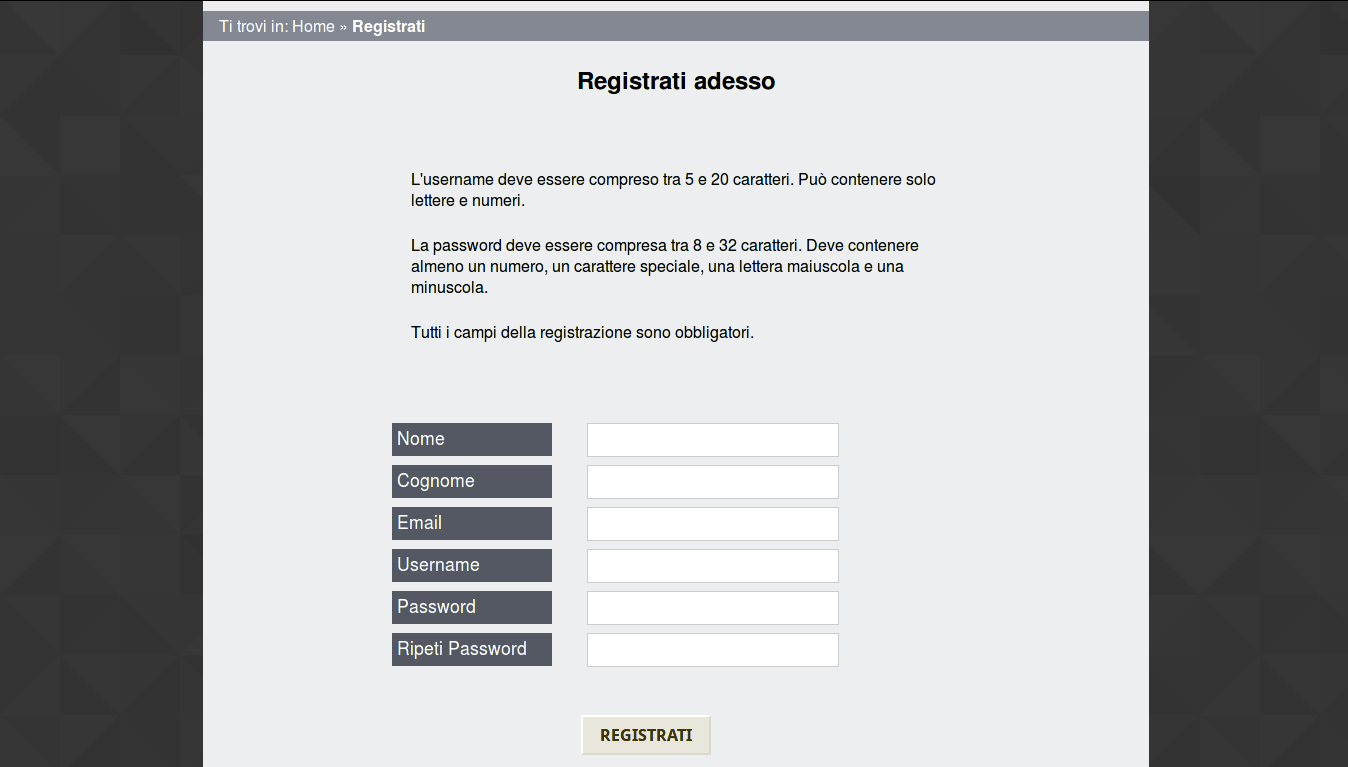
\includegraphics[scale=0.3]{images/protanopia2.jpg}\\[1cm] \caption{Utente affetto da protanopia} 
	\end{figure}
	\begin{figure}
		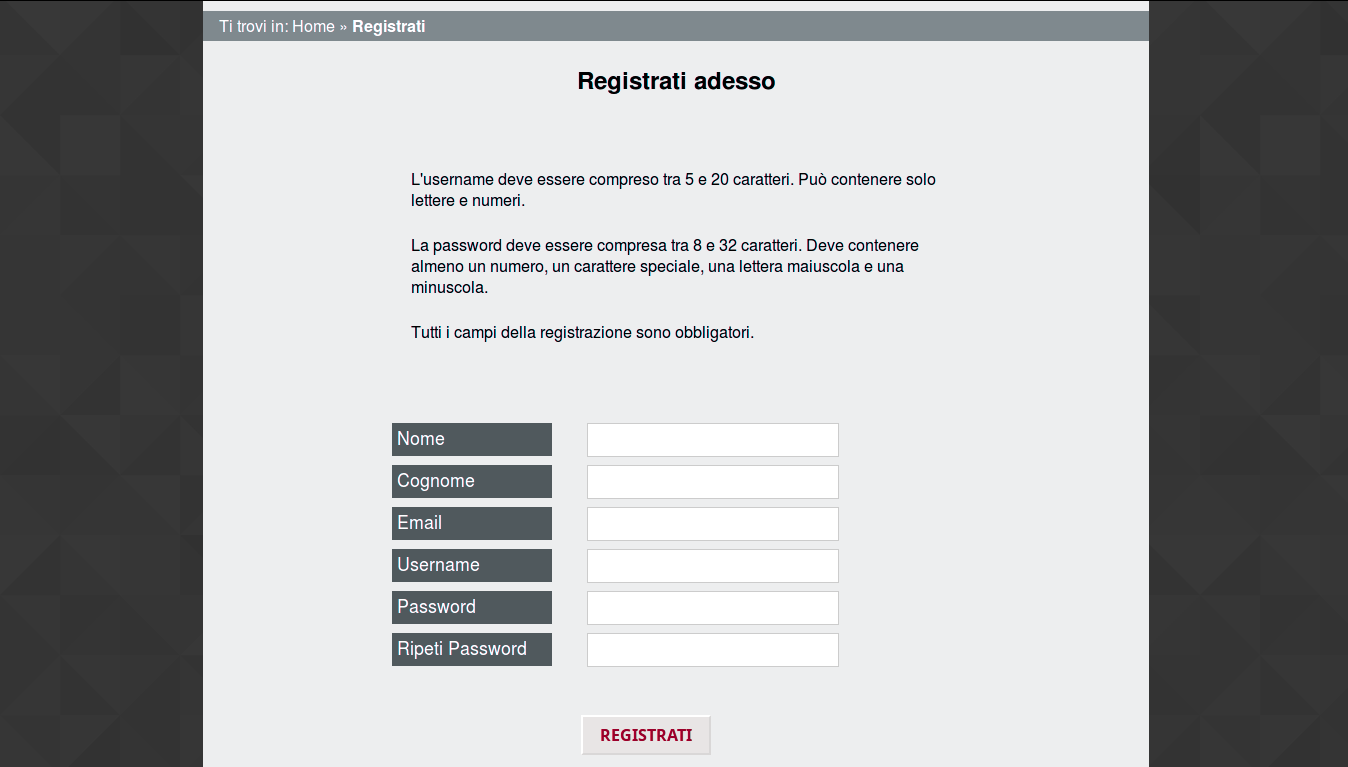
\includegraphics[scale=0.3]{images/tritanopia2.jpg}\\[1cm] \caption{Utente affetto da tritanopia} 
	\end{figure}
	\newpage
	Si può notare che lo schema di colori adottato rende le differenze tra screenshot molto basse.\\
	\subsection{Tag}
	\subsection{Screen reader}
	\subsection{Aiuti per la navigazione}
	\section{Struttura}
	\section{Presentazione}	
	\section{Comportamento}
	Per gestire la parte relativa al comportamento è stato usato JavaScript. In particolare sono stati fatti i seguenti script:
	\begin{itemize}
	\item \textit{controlli.js}: questo script esegue controlli lato client sui dati inseriti durante la registrazione in \textit{registrazione.php}. Tali controlli avvengono ogni volta che l'utente lascia un textfield di inserimento dati tramite l'utilizzo dell'evento \textit{onblur}. Se i dati inseriti non sono validi allora comparirà un messaggio d'errore specifico e ad esso verrà dato il \textit{focus};
	\item \textit{homeslide.js}: questo script permette l'utilizzo dello slideshow presente in \textit{index.php}. È possibile navigare tra le foto dello slideshow utilizzando i pulsanti ai lati, sia con il mouse che con la tastiera, premendo il tasto invio. Per ogni foto dello slideshow è presente inoltre una sua didascalia, la sua posizione rispetto al numero di foto presenti nello slideshow, e un link che porta alla corrispondente foto in \textit{fotoutente.php}. 
	\end{itemize}
	\newpage
	\section{PHP}
	\subsection{Utilizzo}
	Il PHP viene utilizzato per:
	\begin{itemize}
	\item reperire dati dal database(DB) e stamparli;
	\item elaborare dati, presi in input o dal DB, e/o inserirli nel DB.
	\end{itemize} 
	
	Al primo punto appartengono le pagine che si occupano di leggere dati dal DB e stamparli.
	Al secondo punto appartengono le pagine che si occupano puramente di elaborare e/o inserire dati nel DB. Queste pagine sono prive di una GUI, e pertanto non consultabili dagli utenti. Apposite istruzioni di reindirizzamento permettono ciò.
	
	Al primo punto appartengono le pagine nella cartella ....astro/...., che sono:
	\begin{itemize}
	\item \textit{index.php}, che recupera e visualizza le immagini con i miglior rank nel DB e al più 10 tra eventi passati e prossimi;
	\item \textit{listafoto.php}, che recupera e visualizza le principali informazioni su tutte le foto presenti nel DB;
	\item \textit{listastudi.php}, analoga a listafoto.php;
	\item \textit{fotoutente.php?idft=x}, che recupera e visualizza l'immagine(e relative informazioni) con id=x. Inoltre, permette agli utenti loggati di votarla e commentarla;
	\item \textit{studioutente.php?idst=x}, analoga a \textit{fotoutente.php?idft=x};
	\item \textit{eventi.php}, che recupera e visualizza gli eventi passati e futuri nel DB;
	\item \textit{registrazione.php}, che permette all'utente non loggato di inserire i dati per la registrazione al sito. Questa funzione non è disponibile agli utenti loggati;
	\item \textit{login.php}, che permette all'utente non loggato di effettuare l'accesso. Questa funzione non è disponibile agli utenti loggati.
	\end{itemize}
	
	Al secondo punto appartengono le pagine nella cartella ....../astro/backend, che sono:
	\begin{itemize}
	\item \textit{connessione.php}, che tenta la connessione al server e al DB in esso alloggiato. In caso la connessione fallisca, un opportuno messaggio d'errore verrà visualizzato;
	\item \textit{login.php}, che dati mail e password, verifica il tentativo di accesso di un utente, permettendolo o meno. Al fine di proteggersi da SQL injection, la query viene somministrata al DB se e solo se i parametri soddisfano specifiche espressioni regolari. In caso l'accesso non abbia successo (la query ritorna un insieme vuoto o i parametri non soddisfano le regex) viene visualizzato un unico messaggio d'errore;
	\item \textit{logout.php}, che distrugge la sessione;
	\item \textit{registrauser.php}, che dati i parametri di registrazione, verifica se rispettano certe espressioni regolari e se possono essere inserite nel DB (ad esempio non possono esistere due mail uguali). In caso ciò non sia possibile, vengono visualizzati i relativi messaggi d'errore;
	\item \textit{commentafoto.php}, che dato l'id di una foto e un commento inserito da un utente loggato, inserisce nel database il relativo commento(associato all'utente che ha commentato la foto);
	\item \textit{commentastudio.php}, analoga al punto precedente;
	\item \textit{votafoto.php}, analoga a \textit{commentafoto.php}, ma avendo come soggetto un voto e non un commento. Il voto può essere +1 o -1 e, in caso l'utente loggato voti più di una volta la stessa foto, viene eliminato il voto dato precedentemente e inserito quello corrente;
	\item \textit{votastudio.php}, analoga al punto precedente;
	\end{itemize}
	
	Il comportamento delle pagine del sito varia se l'utente è loggato o meno. Questo è reso possibile tramite l'utilizzo delle sessioni. Infatti, se l'accesso ha successo, viene avviata una sessione che memorizza l'utente loggato. Al logout, giustamente, questa sessione viene distrutta. Il comportamento delle pagine varia anche in base ad alcune azioni dell'utente sul database sul quale il sito si appoggia. Ad esempio, vengono segnalati degli errori in caso l'accesso non vada a buon fine.
	
	\subsection{Utente non loggato}
	L'utente non loggato può:
	\begin{itemize}
	\item usare lo slideshow nella pagina iniziale;
	\item consultare gli eventi passati e futuri memorizzati nel database;
	\item consultare la lista delle foto presenti nel database e, tramite pagine apposite, consultare ogni singola foto;
	\item consultare la lista degli studi presenti nel database e, tramite pagine apposite, consultare ogni singolo studio;
	\item consultare la pagina di about, descrittiva dello scopo del sito;
	\item registrarsi al sito;
	\item effettuare l'accesso.
	\end{itemize}
	\subsection{Utente loggato}
	L'utente loggato può:
	\begin{itemize}
	\item fare quello che può fare un utente non loggato, tranne:
	\begin{itemize}
	\item registrarsi al sito;
	\item effettuare l'accesso;
	\end{itemize}
	\item commentare e votare ogni foto;
	\item commentare e votare ogni studio;
	\item effettuare il logout.
	\end{itemize}
	
	\subsection{Sessioni}
	Le sessioni sono usate per due motivi:
	\begin{itemize}
	\item verificare se l'utente è loggato o meno;
	\item generare determinati messaggi d'errore.
	\end{itemize}
	Nel primo caso, quando un utente effettua l'accesso, viene memorizzata la relativa mail(che lo identifica). In caso, tramite sessione, si deduca che l'utente è loggato, vengono erogate le funzionalità aggiuntive. \\ \\
	Nel secondo caso, vengono generati degli opportuni messaggi d'errore relativi ai seguenti casi:
	\begin{itemize}
	\item l'utente non loggato tenta di registrarsi con dei parametri non validi; viene quindi segnalata l'irregolarità relativa al parametro errato;
	\item l'utente non loggato tenta di effettuare l'accesso con dei parametri non validi; viene quindi segnalata l'irregolarità relativa al parametro errato;
	\item l'utente loggato tenta di inserire un commento non valido; viene quindi segnalata l'irregolarità relativa al parametro errato.
	\end{itemize}
	
	\section{Gestione dei dati}
	Per l'organizzazione e memorizzazione dei dati si è fatto affidamento su un DB MySQL. Il DB in questione era stato presentato come progetto per il corso di Basi di dati dell'A.A. 2015-2016 e valutato con 29-30/30 (il voto preciso non è stato comunicato). Il DB è stato quindi esteso/adattato alle esigenze del sito. Tuttavia, alcune relazioni non sono utili al sito, in quanto in origine il DB non era pensato per questo progetto. Nonostante ciò, questo non va a discapito dell'efficienza delle query. Non essendo lo scopo del corso, questa sezione non verrà troppo approfondita, ma verrà comunque fornito uno schema.
	In figura 9 è raffigurato la schema ER della versione iniziale del DB(quella consegnata per il corso di Basi di Dati). In figura 10, invece, sono raffigurate le aggiunte fatte al DB per supportare delle funzionalità del sito.
	Di seguito è riportato un elenco delle principali tabelle utilizzate:
	\newpage
	\begin{itemize}
		\item astrofilo: contiene i dati di registrazione dell'utente;
		\item evento: contiene i tipi d'evento che possono essere studiati;
		\item avvenimento: contiene gli eventi che avverranno o sono avvenuti;
		\item corpo: contiene i tipi di corpo studiabili;
		\item studia: contiene i dati degli studi;
		\item foto: contiene i dati sulle foto;
		\item giudicastudio(foto): contiene i voti dati dagli astrofili a tutti gli studi(foto);
		\item commentastudio(foto): contiene i commenti degli astrofili di ogni studio(foto);
	\end{itemize}
	\begin{figure}
		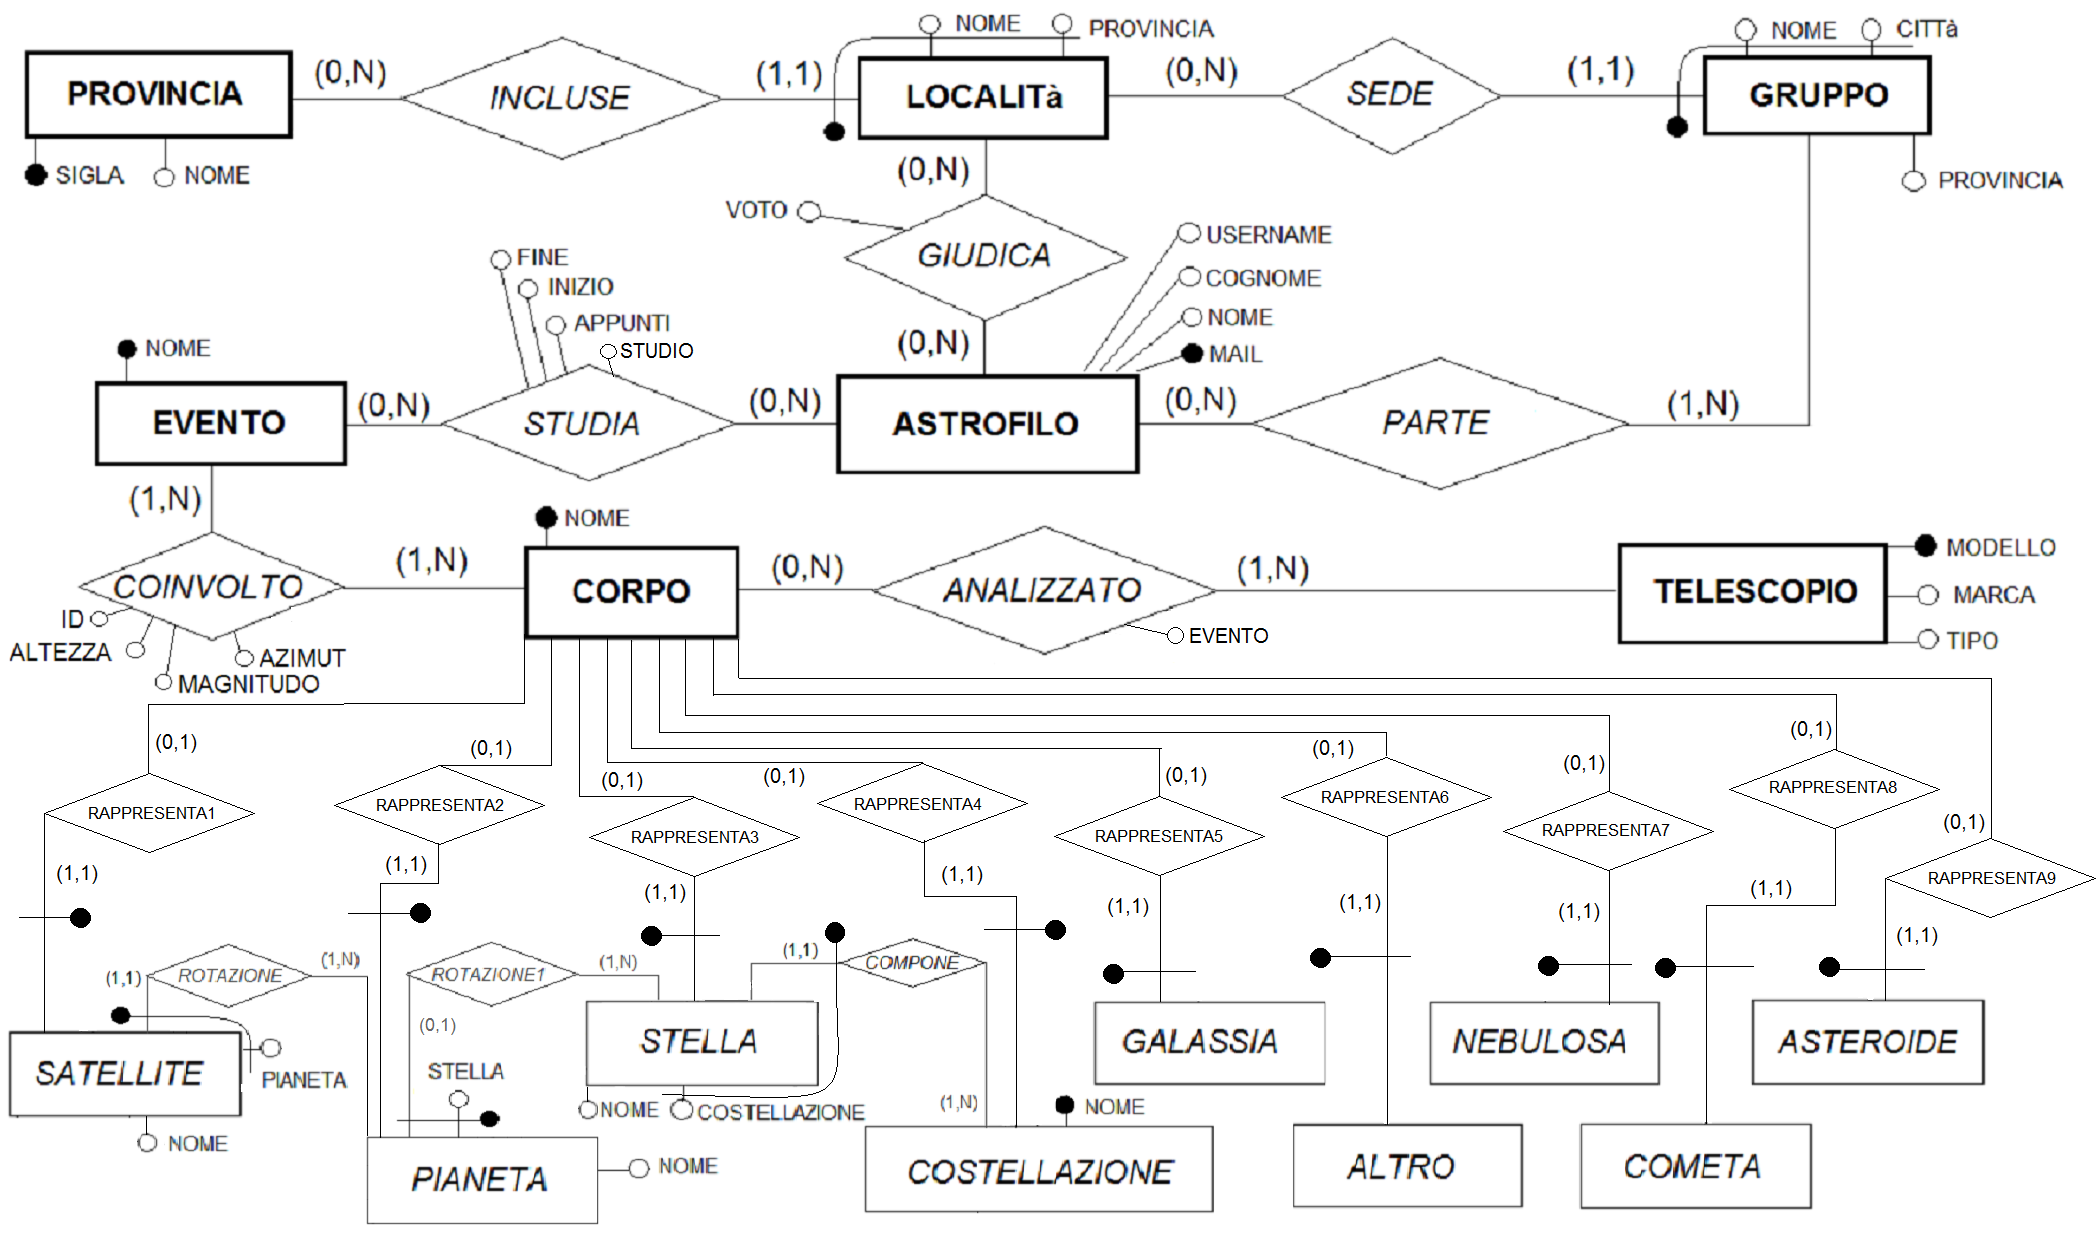
\includegraphics[scale=0.2]{images/ERR-FINITO.png}\\[1cm] \caption{DB iniziale.}
	\end{figure}
	\begin{figure}
		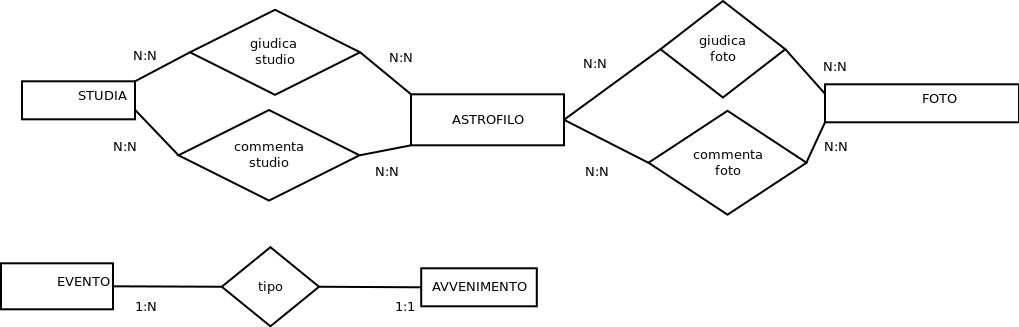
\includegraphics[scale=0.35]{images/DBplus.png}\\[1cm] \caption{Aggiunte al DB iniziale}
	\end{figure}
	\newpage
	\section{Test}
	\subsection{Validazione}
	Per la validazione, è stato usato il validatore online messo a disposizione da W3C. Per validare ogni pagina, si sono seguiti i seguenti passi:
	\begin{itemize}
		\item esecuzione del file nel browser;
		\item copia del codice sorgente(tasto dx + view source code);
		\item dato in pasto al validatore il codice tramite "validate by input".
	\end{itemize}
	Tutte le pagine e i file CSS hanno superato questo test.
	\subsection{Browser}
	Senza riscontrare grosse differenze, il sito è stato fatto girare su:
	\begin{itemize}
		\item Mozilla Firefox 39.0, 51.0.1;
		\item Chromium 55.0;
		\item Google Chrome;
		\item Internet Explorer;
		
	\end{itemize}
	e sui seguenti sistemi operativi:
	\begin{itemize}
		\item Linux Mint 18.1;
		\item Ubuntu 14.04;
		\item Windows 10;
		\item MAC??
	\end{itemize}
	\subsubsection{JavaScript}
	che succede senza JS?
	\subsubsection{PHP}
	Sono stati fatti dei test di usabilità nel caso non sia possibile connettersi al DB. Il risultato è che il sito non può offrire le funzionalità che si prefigge, ma resta comunque navigabile.
	\section{Suddivisione ruoli}
	Il gruppo si è suddiviso il lavoro in maniera equa sulle parti di struttura, presentazione, comportamento e accessibilità.
	Ognuno dei membri si è occupato di tutte le parti, tuttavia abbiamo ritenuto intelligente che ogni membro si concentrasse maggiormente su una specifica parte.
	I ruoli sono stati così ripartiti:
	\begin{itemize}
		\item struttura: tutti i membri del gruppo;
		\item presentazione: Andrea Magnan, Matteo Slanzi(anche gli altri membri hanno contribuito, ma in forma minore);
		\item comportamento: Mattia Bottaro(PHP), Andrea Magnan(JS)(anche gli altri membri hanno contribuito, ma in forma minore);
		\item accessibilità: Riccardo Saggese, Matteo Slanzi(anche gli altri membri hanno contribuito, ma in forma minore)
	\end{itemize}
\end{document}